% npj Digital Surgery -- Article
% Format per npj Series content types:
%   Title <= 15 words, free of punctuation, idioms and puns
%   Abstract <= 150 words, no subheadings
%   Introduction: no subheadings
%   Results: subheadings used
%   Discussion: no subheadings, and no Limitations or Conclusions sections
%   Methods: subheadings used, in the main file
%   Data availability mandatory; Code availability where applicable
%   References limited to 60
%
% Every numeric value is pulled from macros.tex, generated by
% scripts/13_make_macros.py from the result CSVs, so the text cannot drift
% from the experiments.
\documentclass[11pt]{article}
\usepackage[margin=1in]{geometry}
\usepackage{graphicx,booktabs,amsmath,siunitx,microtype}
\usepackage{tabularx}
\usepackage[hidelinks]{hyperref}
% xurl must follow hyperref: it permits line breaks at any character in a URL,
% without which long repository and DOI links overrun the right margin.
\usepackage{xurl}
\usepackage[round]{natbib}
\graphicspath{{../outputs/figures/}}
% Generated by scripts/13_make_macros.py -- do not edit by hand.
% Every number quoted in the manuscript is defined here from the result CSVs.

\newcommand{\BlockDice}{0.8534}
\newcommand{\BlockGap}{+0.1317}
\newcommand{\CVCThreeMatched}{60}
\newcommand{\ClusterARI}{0.497}
\newcommand{\DiversityEstimate}{0.0269}
\newcommand{\ExtClinicMax}{0.0382}
\newcommand{\ExtClinicMin}{0.0198}
\newcommand{\ExtKvasirMax}{0.0183}
\newcommand{\ExtKvasirMin}{0.0027}
\newcommand{\IdentityMaxDiff}{1.9e-06}
\newcommand{\InflationAdjusted}{0.0701}
\newcommand{\InflationAdjustedSigma}{13.2}
\newcommand{\InflationClinic}{0.0970}
\newcommand{\InflationClinicClean}{0.8231}
\newcommand{\InflationClinicHi}{0.1031}
\newcommand{\InflationClinicLo}{0.0911}
\newcommand{\InflationClinicModelMax}{0.1180}
\newcommand{\InflationClinicModelMin}{0.0800}
\newcommand{\InflationClinicN}{612}
\newcommand{\InflationClinicPairs}{3,060}
\newcommand{\InflationClinicRandom}{0.9201}
\newcommand{\InflationClinicSigma}{18.3}
\newcommand{\InflationClinicSigmaMax}{22.3}
\newcommand{\InflationClinicSigmaMin}{15.1}
\newcommand{\InflationKvasir}{0.0059}
\newcommand{\InflationKvasirClean}{0.8996}
\newcommand{\InflationKvasirHi}{0.0086}
\newcommand{\InflationKvasirLo}{0.0033}
\newcommand{\InflationKvasirModelMax}{0.0105}
\newcommand{\InflationKvasirModelMin}{0.0024}
\newcommand{\InflationKvasirN}{1,000}
\newcommand{\InflationKvasirPairs}{5,000}
\newcommand{\InflationKvasirRandom}{0.9055}
\newcommand{\InflationKvasirSigma}{1.1}
\newcommand{\InflationKvasirSigmaMax}{2.0}
\newcommand{\InflationKvasirSigmaMin}{0.4}
\newcommand{\NCVCThree}{60}
\newcommand{\NClinic}{612}
\newcommand{\NColon}{380}
\newcommand{\NDupesCVCThree}{2}
\newcommand{\NDupesClinic}{0}
\newcommand{\NDupesColon}{34}
\newcommand{\NDupesEtis}{3}
\newcommand{\NDupesKvasir}{0}
\newcommand{\NDupesSessile}{0}
\newcommand{\NEtis}{196}
\newcommand{\NKvasir}{1000}
\newcommand{\NPairs}{10}
\newcommand{\NRuns}{100}
\newcommand{\NSessile}{196}
\newcommand{\NSignFlips}{1}
\newcommand{\NUniqueCVCThree}{58}
\newcommand{\NUniqueClinic}{612}
\newcommand{\NUniqueColon}{346}
\newcommand{\NUniqueEtis}{193}
\newcommand{\NUniqueKvasir}{1000}
\newcommand{\NUniqueSessile}{196}
\newcommand{\NearDupNinetyCVCThree}{83.3}
\newcommand{\NearDupNinetyClinic}{90.0}
\newcommand{\NearDupNinetyColon}{85.8}
\newcommand{\NearDupNinetyEightCVCThree}{55.0}
\newcommand{\NearDupNinetyEightClinic}{23.4}
\newcommand{\NearDupNinetyEightColon}{38.2}
\newcommand{\NearDupNinetyEightEtis}{40.3}
\newcommand{\NearDupNinetyEightKvasir}{0.8}
\newcommand{\NearDupNinetyEightSessile}{1.0}
\newcommand{\NearDupNinetyEtis}{77.5}
\newcommand{\NearDupNinetyFiveCVCThree}{80.0}
\newcommand{\NearDupNinetyFiveClinic}{57.5}
\newcommand{\NearDupNinetyFiveColon}{67.4}
\newcommand{\NearDupNinetyFiveEtis}{56.6}
\newcommand{\NearDupNinetyFiveKvasir}{1.2}
\newcommand{\NearDupNinetyFiveSessile}{2.0}
\newcommand{\NearDupNinetyKvasir}{15.3}
\newcommand{\NearDupNinetySessile}{12.2}
\newcommand{\NimagesTotal}{2,248}
\newcommand{\PraNetAvgThree}{0.7429}
\newcommand{\PraNetAvgTwo}{0.6760}
\newcommand{\PraNetBlock}{0.8767}
\newcommand{\PraNetBlockDiff}{1.9e-06}
\newcommand{\PraNetBlockGap}{+0.1916}
\newcommand{\PraNetCVCThree}{0.8767}
\newcommand{\PraNetClinicAll}{0.9697}
\newcommand{\PraNetColon}{0.7153}
\newcommand{\PraNetEtis}{0.6367}
\newcommand{\PraNetRest}{0.6851}
\newcommand{\PraNetShift}{-0.0669}
\newcommand{\PraNetShiftSigma}{12.6}
\newcommand{\PriorClinic}{0.2982}
\newcommand{\PriorColon}{0.2166}
\newcommand{\PriorEtis}{0.1599}
\newcommand{\PriorKvasir}{0.3963}
\newcommand{\PriorPctClinic}{36}
\newcommand{\PriorPctColon}{30}
\newcommand{\PriorPctEtis}{24}
\newcommand{\PriorPctKvasir}{44}
\newcommand{\PriorTrainedClinic}{0.8231}
\newcommand{\PriorTrainedColon}{0.7199}
\newcommand{\PriorTrainedEtis}{0.6611}
\newcommand{\PriorTrainedKvasir}{0.8996}
\newcommand{\RankMovedClinic}{0}
\newcommand{\RankMovedKvasir}{2}
\newcommand{\RecoveryARI}{0.997}
\newcommand{\RecoveryBoundaryF}{1.000}
\newcommand{\RescoreMaxShift}{0.0252}
\newcommand{\RescoreMaxSigma}{4.8}
\newcommand{\RescoreMinShift}{0.0138}
\newcommand{\RescoreMinSigma}{2.6}
\newcommand{\RescoreNModels}{5}
\newcommand{\RescoreNShifted}{5}
\newcommand{\RestDice}{0.7216}
\newcommand{\SafeHomogeneity}{0.953}
\newcommand{\SafeKRatio}{0.041}
\newcommand{\SessileMatchedCorr}{196}
\newcommand{\SessileMatchedPhash}{196}
\newcommand{\SessileMatchedPhashExact}{155}
\newcommand{\SessileMatchedPixel}{0}
\newcommand{\SessileN}{196}
\newcommand{\SigmaRun}{0.0053}
\newcommand{\TopCorrected}{segformer\_b2}
\newcommand{\TopPublished}{unet\_pvt}


\title{\textbf{Duplicate images and leaking splits in public polyp segmentation benchmarks}}
% Affiliation is listed as independent because the work was carried out
% independently of the author's employment, which is disclosed in full under
% Competing interests. To attribute the work to the employer instead, replace
% the line below -- but obtain written publication clearance first.
\author{Rishit Puri\\[2pt]
\normalsize Independent researcher\\
\normalsize ORCID \href{https://orcid.org/0009-0004-6215-9997}{0009-0004-6215-9997}\\
\normalsize \texttt{rishitpuri15@gmail.com}}
\date{}

\begin{document}
\maketitle

\begin{abstract}
\noindent
Automated polyp segmentation is benchmarked almost exclusively on a small set
of public datasets distributed together as one evaluation suite. We audit
those artifacts at the image level. All \CVCThreeMatched{} CVC-300 images are
pixel-identical to CVC-ColonDB frames, so the two are not independent test
sets; \NDupesColon{} of \NColon{} CVC-ColonDB files are exact duplicates of
other files in the same folder; and the distributed CVC-ColonDB cannot be
reconciled with its published specification of 300 frames selected to
maximise visual difference. Correcting the double counting shifts every
architecture's mean external Dice by \RescoreMinSigma--\RescoreMaxSigma{}
times the protocol's measured run-to-run noise floor and reverses which
architecture ranks first. Frames are redundant enough that every random split
of CVC-ClinicDB leaks, inflating in-domain Dice by \InflationClinic{}
(\InflationClinicSigma$\sigma$), whereas Kvasir-SEG inflates by only
\InflationKvasir{}. We release leakage-free splits, recovered sequence labels
and the audit code.
\end{abstract}

\section*{Introduction}

% No subheadings permitted in this section.
Progress in automated polyp segmentation is reported almost entirely through a
single evaluation template. A model is trained on Kvasir-SEG and
CVC-ClinicDB, then scored on CVC-ColonDB, ETIS-LaribPolypDB and CVC-300, and
the five resulting Dice values are compared against a leaderboard inherited
from PraNet~\citep{fan2020pranet}. Recent work has begun to ask what that
template can establish. Reported differences between architectures can fall
below the run-to-run variance of the training procedure
itself~\citep{puri2026what}, split protocols that co-exist in the literature
are mutually incomparable, and near-tied rankings reverse when the partition
is redrawn~\citep{urooj2026metrics}. General guidance on validation practice
has been issued for medical image analysis as a
whole~\citep{maierhein2024metrics}, but it presumes that the datasets under
evaluation are what their documentation says they are.

Those critiques treat the datasets as given and ask whether the statistics
computed on them are sound. We ask the prior question of whether the artifacts
themselves are what they are believed to be. This is not a hypothetical
concern: duplicate and near-duplicate images have been shown to contaminate
widely used dermatology benchmarks and to change the conclusions drawn from
them~\citep{cassidy2022isic,groger2023dermatology}, and the colonoscopy
datasets have a structural reason to be vulnerable. Every one of them is
assembled from frames extracted from a small number of colonoscopy videos, so
visually near-identical frames are available in abundance, and most of the
datasets never published a mapping from frame to source video.

We audit the suite at the level of individual images and report three classes
of finding. First, the suite contains redundancy that is invisible to the
protocol: one test set is contained in another, several files are exact
duplicates, and the proportion of images carrying a near-duplicate reaches
\NearDupNinetyClinic\% in CVC-ClinicDB against
\NearDupNinetyKvasir\% in Kvasir-SEG. Second, the circulating CVC-ColonDB
cannot be reconciled with the dataset its creators describe, and the
authoritative copy needed to reconcile them is no longer obtainable. Third,
these defects are consequential rather than cosmetic: they move reported
scores and architecture rankings by multiples of the noise floor that the same
protocol exhibits under repeated identical training.

Throughout we report effects in units of $\sigma_{\mathrm{run}} =
\SigmaRun{}$ Dice, the run-to-run noise floor measured for this training
recipe~\citep{puri2026what,puri2026data}, because an effect that cannot be
distinguished from rerunning the same configuration cannot support a claim. We release
leakage-free splits, recovered sequence labels, per-image results for all
\NRuns{} training runs, and the audit code.

\section*{Results}

\subsection*{One external test set is contained in another}

% Tier 1 claim: identity, verifiable by arithmetic rather than inference.
Table~\ref{tab:audit} summarises the audit and Table~\ref{tab:effects} the
consequences measured from it.

Across the \NimagesTotal{} images of the suite, every one of the
\CVCThreeMatched{} CVC-300 images is pixel-identical to an image in
CVC-ColonDB, occupying the contiguous frame range 149--208
(Fig.~\ref{fig:contamination}a). Agreement holds under two independent
criteria, MD5 of the decoded pixel array and a 256-bit perceptual hash at zero
Hamming distance. A third, fully independent check confirms it downstream:
scored by five trained architectures, CVC-300 and CVC-ColonDB frames
149--208 yield mean Dice agreeing to within \IdentityMaxDiff{}.

Consequently CVC-300 and CVC-ColonDB are not independent test sets, and
averaging them as separate datasets counts those \CVCThreeMatched{} images
twice. The duplicated block is also unrepresentative of its parent: it scores
\BlockDice{} against \RestDice{} for the remainder of CVC-ColonDB, a gap of
\BlockGap{} Dice. Reporting it separately therefore counts an unusually easy
subset twice.

\begin{table}[t]\centering
\caption{\textbf{Image-level audit of the evaluation suite.} Files counts the
images as distributed; Unique counts distinct images by the MD5 digest of the
decoded pixels. Kvasir-Sessile is distributed separately and its images are
drawn from Kvasir-SEG, so it is excluded from suite totals.}
\label{tab:audit}
\small
\begin{tabular}{lrrrrrl}
\toprule
Dataset & Files & Unique & Exact & \multicolumn{2}{c}{Near-duplicate (\%)} & Contained in \\
\cmidrule(lr){5-6}
 & & & dupl. & $r>0.95$ & $r>0.90$ & \\
\midrule
Kvasir-SEG & 1000 & 1000 & 0 & 1.2 & 15.3 & -- \\
Kvasir-Sessile & 196 & 196 & 0 & 2.0 & 12.2 & Kvasir-SEG \\
CVC-ClinicDB & 612 & 612 & 0 & 57.5 & 90.0 & -- \\
CVC-ColonDB & 380 & 346 & 34 & 67.4 & 85.8 & -- \\
CVC-300 & 60 & 58 & 2 & 80.0 & 83.3 & CVC-ColonDB \\
ETIS-Larib & 196 & 193 & 3 & 56.6 & 77.5 & -- \\
\bottomrule
\end{tabular}

\end{table}

\subsection*{Exact duplicates and pervasive near-duplication}

CVC-ColonDB contains \NDupesColon{} files that are byte-level duplicates of
other files in the same folder, leaving \NUniqueColon{} unique images among
\NColon{}; ETIS-LaribPolypDB contains \NDupesEtis{}. Beyond exact copies,
the proportion of images possessing a near-duplicate within the same dataset
is \NearDupNinetyClinic\% for CVC-ClinicDB, \NearDupNinetyColon\% for
CVC-ColonDB and \NearDupNinetyEtis\% for ETIS-LaribPolypDB, against
\NearDupNinetyKvasir\% for Kvasir-SEG (Fig.~\ref{fig:contamination}b).

The audit also returns negative results that bound its scope. No image is
shared between Kvasir-SEG and any CVC dataset, CVC-ClinicDB and CVC-ColonDB
share no images despite common provenance, and ETIS-LaribPolypDB is clean
against every other set.

\subsection*{A second containment is invisible to exact hashing}

Kvasir-Sessile is distributed separately from Kvasir-SEG and is sometimes
treated as a held-out set of flat and sessile lesions. All \SessileN{} of its
images correspond to a Kvasir-SEG image: they share filenames, have identical
dimensions, and match at a thumbnail correlation above $0.999$ in
\SessileMatchedCorr{} of \SessileN{} cases and at a perceptual-hash distance
of at most five bits in \SessileMatchedPhash{}. Kvasir-Sessile is therefore
contained in Kvasir-SEG, and using it as a test set for a model trained on
Kvasir-SEG admits the whole of it into training.

The two containments are nonetheless detected very differently
(Fig.~\ref{fig:contamination}c). CVC-300 is recovered completely by every
signal, including the MD5 digest of the decoded pixels. Kvasir-Sessile is
recovered completely by correlation and by perceptual hashing at a tolerance
of five bits, by \SessileMatchedPhashExact{} of \SessileN{} at zero
perceptual-hash distance, and by \SessileMatchedPixel{} of \SessileN{} by
exact pixel digest, because the images were re-encoded between the two
releases. An audit resting on checksums alone would report this dataset as
clean. Duplicate detection in benchmark suites therefore cannot rely on exact
hashing, a point that applies well beyond the datasets examined here.

\begin{figure}[t]\centering
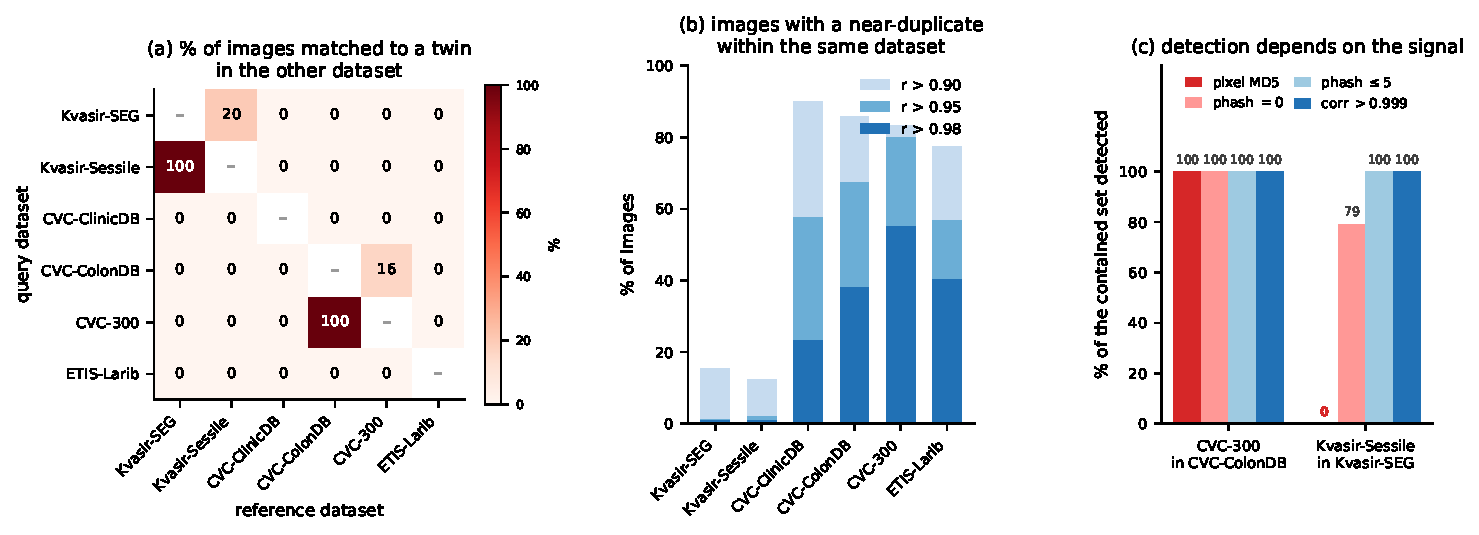
\includegraphics[width=\textwidth]{fig1_contamination.pdf}
\caption{\textbf{What the benchmark suite contains.}
(a) Percentage of each dataset's images matched to a twin in another dataset,
under the criterion that the correlation and perceptual-hash signals agree.
(b) Percentage having a near-duplicate within the same dataset at three
correlation thresholds. (c) Proportion of each contained set recovered by
four detection signals; exact pixel hashing recovers none of Kvasir-Sessile.}
\label{fig:contamination}
\end{figure}

\subsection*{The distributed CVC-ColonDB cannot be reconciled with its specification}

% Deliberately framed as a reconciliation failure, not as corruption: we
% cannot inspect the authoritative copy, so we cannot assert what the
% surplus images are.
The CVC-ColonDB that circulates in the evaluation suite differs from the
dataset its creators describe. The authoritative project page specifies
15 short colonoscopy sequences from 15 studies, with region-of-interest
annotations provided for 300 frames, distributed as 1200 files comprising the
originals and three mask types. Those 300 frames are stated to have been
``selected in order to maximise the visual difference between them''.

The copy distributed with the benchmark suite contains \NColon{} image files,
of which \NUniqueColon{} are unique. Neither figure matches the specified 300,
and the surplus cannot be characterised: the download host specified by the
creators has been unreachable, the page itself has not been revised since
2018, and neither the archive nor the registration endpoint was ever captured
by the Internet Archive, so no authoritative copy remains against which to
reconcile the difference. We therefore report the discrepancy without
attributing a cause.

The curation statement is nonetheless directly testable against the
circulating artifact, and it does not hold: \NearDupNinetyColon\% of the
distributed images carry a near-duplicate at $r > 0.90$ and
\NDupesColon{} are pixel-identical copies. Whatever the \NColon{}-file
artifact is, it is not a set of frames selected to maximise visual
difference. Because the authoritative copy is unobtainable, this is also a
plausible explanation for how the discrepancy has persisted unremarked: there
has been nothing to check against.

\subsection*{The containment affects the model that defined the protocol}

The results so far concern architectures we trained ourselves. Because PraNet
released both the protocol and its trained weights, the containment can be
examined on the model the field actually cites, with no retraining and
without our training recipe entering the comparison. Running the released
checkpoint over the same images reproduces the published figures closely,
giving \PraNetColon{} on CVC-ColonDB, \PraNetEtis{} on ETIS-LaribPolypDB and
\PraNetCVCThree{} on CVC-300 against the \num{0.709}, \num{0.628} and
\num{0.871} reported, which indicates that the evaluation pipeline used here
is faithful.

On that checkpoint, CVC-300 and CVC-ColonDB frames 149--208 yield mean Dice
differing by \PraNetBlockDiff{}, and the duplicated block scores
\PraNetBlock{} against \PraNetRest{} for the remainder of CVC-ColonDB, a gap
of \PraNetBlockGap{} Dice. The protocol presents three unseen datasets, but
two of them are the same images, and the easier of the two subsets is counted
twice. Averaging the three as reported gives \PraNetAvgThree{}; averaging the
two that are genuinely distinct gives \PraNetAvgTwo{}, a difference of
\PraNetShift{} Dice, or \PraNetShiftSigma$\sigma_{\mathrm{run}}$. The claim
supported by this protocol is generalisation to two unseen datasets rather
than three.

CVC-ClinicDB is excluded from that average because the checkpoint was trained
on 550 of its 612 images, so it is not a held-out set for this model.
Evaluating it on all 612 regardless returns \PraNetClinicAll{} against the
\num{0.899} reported for the 62 images actually held out, which indicates the
size of the gap that scoring a model on its own training data can produce.

\begin{table}[t]\centering
\caption{\textbf{Measured consequences, in Dice and in units of the
run-to-run noise floor} $\sigma_{\mathrm{run}} = \SigmaRun{}$. Negative
values indicate that the corrected figure is lower than the reported one.
The position prior is an absolute score rather than a difference, so no
noise-floor ratio is given.}
\label{tab:effects}
\small
\begin{tabular}{lrrl}
\toprule
Effect & Dice & $/\sigma_{\mathrm{run}}$ & Note \\
\midrule
Dropping CVC-300 from the suite average (5 architectures) & -0.0214 & 4.0 & top rank reverses; 2/5 move \\
Dropping CVC-300, released PraNet checkpoint & -0.0669 & 12.6 & three unseen datasets become two \\
Random vs sequence-disjoint splits, CVC-ClinicDB & +0.0970 & 18.3 & 612 frames $\times$ 5 arch., paired, $p<10^{-60}$ \\
\quad adjusted for training diversity & +0.0701 & 13.2 & estimate, see text \\
Random vs grouped splits, Kvasir-SEG & +0.0059 & 1.1 & 3/5 intervals cross zero \\
Content-free position prior, Kvasir-SEG & 0.3963 & -- & vs 0.8996 trained \\
Content-free position prior, CVC-ClinicDB & 0.2982 & -- & vs 0.8231 trained \\
\bottomrule
\end{tabular}

\end{table}

\subsection*{Correcting the double counting reverses the leading architecture}

Recomputing the benchmark from per-image metrics for five architectures under
five-fold cross-validation, with CVC-300 removed as a duplicate of
CVC-ColonDB and exact duplicates collapsed, shifts mean external Dice by
\RescoreMinShift--\RescoreMaxShift{} Dice, that is
\RescoreMinSigma--\RescoreMaxSigma$\sigma_{\mathrm{run}}$, for
\RescoreNShifted{} of \RescoreNModels{} architectures. The ordering changes:
\TopPublished{} ranks first under the published four-dataset average and
\TopCorrected{} ranks first once the duplication is removed
(Fig.~\ref{fig:cvcthree}). \NSignFlips{} of \NPairs{} pairwise comparisons
change sign, and it is the comparison that decides the leading architecture.

\begin{figure}[t]\centering
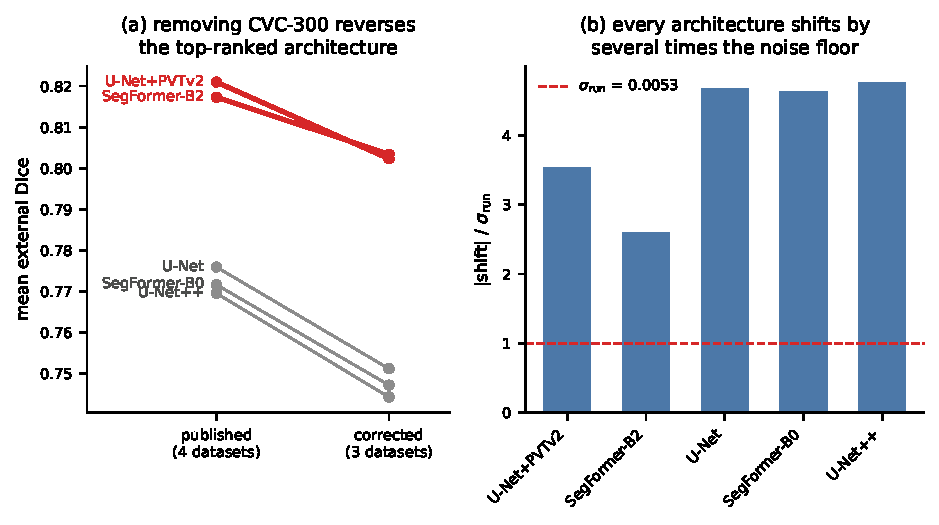
\includegraphics[width=\textwidth]{fig2_cvc300_double_counting.pdf}
\caption{\textbf{Consequence of counting CVC-300 as an independent test set.}
(a) Mean external Dice before and after removing the duplication; the
architectures that exchange rank are highlighted. (b) Magnitude of the shift
in units of $\sigma_{\mathrm{run}}$.}
\label{fig:cvcthree}
\end{figure}

\subsection*{Leaking splits inflate CVC-ClinicDB by eighteen noise floors}

Near-duplication within a training set has a direct consequence: a random
assignment of frames to folds places visually near-identical frames on both
sides of the partition. Using the official frame-range table, which assigns
each of CVC-ClinicDB's 612 frames to one of 29 source sequences, every one of
1000 random 80/20 partitions placed frames from all of the test sequences in
the training set as well.

We trained five architectures over five folds under one recipe twice: once
with frames assigned at random, as the literature does, and once with whole
source sequences held out. Both arms partition all \InflationClinicN{} frames,
so every frame is held out exactly once per protocol and the two arms can be
compared on identical images rather than on different test folds, giving
\InflationClinicPairs{} paired observations across the five architectures.
Random
splits yield a mean Dice of \InflationClinicRandom{} against
\InflationClinicClean{} for sequence-disjoint splits, an inflation of
\InflationClinic{} Dice [\InflationClinicLo, \InflationClinicHi], or
\InflationClinicSigma$\sigma_{\mathrm{run}}$. The effect is present in every
architecture (\InflationClinicModelMin--\InflationClinicModelMax{} Dice,
\InflationClinicSigmaMin--\InflationClinicSigmaMax$\sigma$) and is far larger
than the spread between architectures (Fig.~\ref{fig:inflation}a).

Repeating the comparison on Kvasir-SEG, whose near-duplicate rate is
\NearDupNinetyKvasir\% rather than \NearDupNinetyClinic\%, yields an
inflation of \InflationKvasir{} Dice, or
\InflationKvasirSigma$\sigma_{\mathrm{run}}$, with intervals crossing zero for
three of five architectures (Fig.~\ref{fig:inflation}b). The magnitude of the
effect therefore tracks the redundancy of the dataset rather than the choice
of partitioning procedure in itself.

Part of the in-domain difference is not leakage. Scores on the external test
sets, which neither arm trained on, also differ between the arms by
\ExtClinicMin--\ExtClinicMax{} Dice. Leakage cannot act on data that was never
seen, and the two arms differ in a second respect: at equal training-set size,
the sequence-disjoint folds exclude roughly a fifth of the source sequences
and so present fewer distinct lesions. Taking the mean external difference
\DiversityEstimate{} as an estimate of that contribution gives an adjusted
in-domain estimate of \InflationAdjusted{} Dice, or
\InflationAdjustedSigma$\sigma_{\mathrm{run}}$, attributable to leakage
proper. The corresponding external differences in the Kvasir-SEG experiment,
where grouping removes almost no lesion diversity, are
\ExtKvasirMin--\ExtKvasirMax{} Dice, which is consistent with this account.

Unlike the duplication of CVC-300, leakage did not change the in-domain
ordering of architectures on CVC-ClinicDB, where \RankMovedClinic{} of
\RescoreNModels{} architectures moved. On Kvasir-SEG, where the mean effect is
at the noise floor, \RankMovedKvasir{} of \RescoreNModels{} moved, because the
two leading architectures are separated by less than
$\sigma_{\mathrm{run}}$. A shift in the mean and a change in the ranking are
distinct failures, and neither implies the other.

\begin{figure}[t]\centering
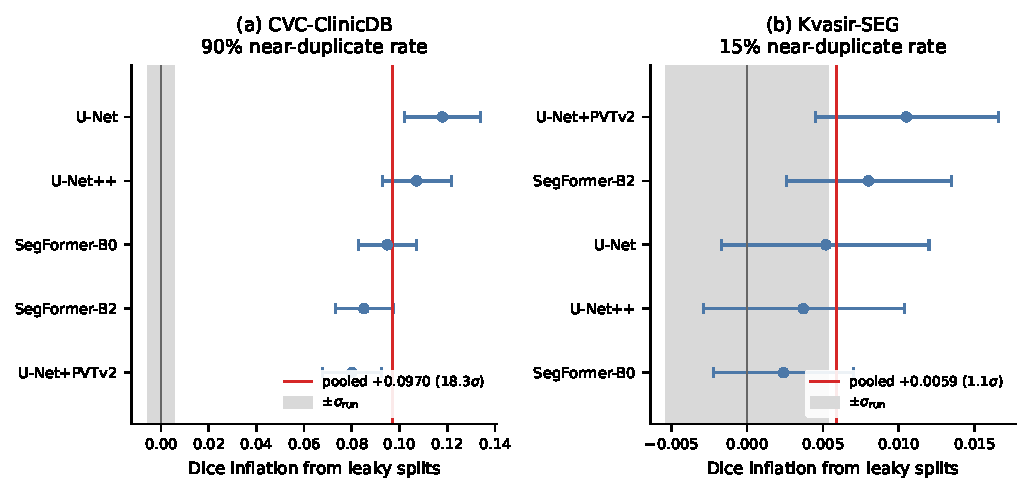
\includegraphics[width=\textwidth]{fig3_leakage_inflation.pdf}
\caption{\textbf{Inflation attributable to leaking splits.}
Per-architecture inflation with percentile bootstrap intervals, pooled
estimate in red and the $\pm\sigma_{\mathrm{run}}$ band shaded, for
(a) CVC-ClinicDB and (b) Kvasir-SEG.}
\label{fig:inflation}
\end{figure}

\subsection*{A predictor that never sees the image}

Benchmark polyps are typically centred and well framed, a bias previously
reported as a dataset statistic~\citep{ji2024vps}. To express that bias in the
metric the field reports, we constructed a predictor that sees no image
content: it averages the training-fold masks into a single probability map,
thresholds it at the value maximising training Dice, and emits that one fixed
shape for every test image.

The prior alone reaches \PriorKvasir{} Dice on Kvasir-SEG and \PriorClinic{}
on CVC-ClinicDB, against \PriorTrainedKvasir{} and \PriorTrainedClinic{} for
models trained under the leak-free protocol (Fig.~\ref{fig:prior}a). Values
across the four datasets are ordered exactly by mean lesion area
(Fig.~\ref{fig:prior}b), which identifies the mechanism: a single fixed blob
overlaps large, centrally framed lesions and misses small or peripheral ones.
Dice is not linear in task difficulty, so these figures should not be read as
a fraction of the problem solved. They establish a floor below which a
reported score carries no evidence of lesion recognition at all, and on the
two datasets used for training and in-domain reporting that floor is near
\PriorClinic--\PriorKvasir{}.

\begin{figure}[t]\centering
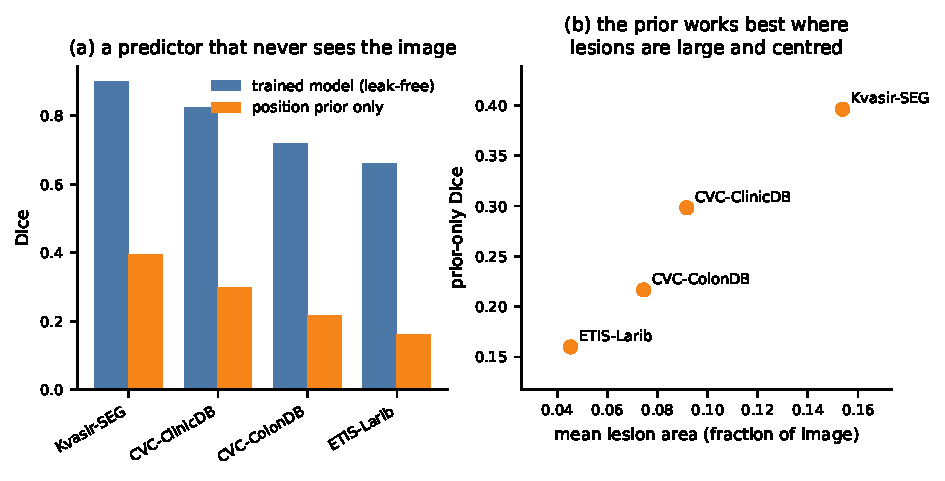
\includegraphics[width=\textwidth]{fig4_position_prior.pdf}
\caption{\textbf{Dice obtainable without seeing the image.}
(a) Trained models against a content-free position prior. (b) Prior-only Dice
against mean lesion area.}
\label{fig:prior}
\end{figure}

\subsection*{Source video structure is recoverable from pixels}

Leakage-free partitioning requires knowing which frames share a source video,
and most of these datasets never published that mapping. It is nonetheless
recoverable. Because frames from one sequence occupy a contiguous range of the
distributed numbering, recovery is a segmentation problem on an ordered
stream rather than a clustering problem. Partitioning CVC-ClinicDB into
contiguous segments that minimise within-segment feature variance recovers the
29 official sequences at an adjusted Rand index of \RecoveryARI{}, with
boundaries located to within two frames at an F1 of \RecoveryBoundaryF{}
(Fig.~\ref{fig:recovery}). Treating the same problem as unordered clustering
reaches only \ClusterARI{}, and thresholding a similarity graph fails
outright because the graph percolates into a single component.

Exact recovery is not in fact required. The two error directions are not
symmetric: splitting one true sequence across groups permits leakage, whereas
merging two sequences into one group does not, costing only partitioning
granularity. The quantity to control is therefore completeness rather than
agreement, and a deliberately coarse segmentation satisfies it. On
CVC-ClinicDB no true sequence is split for any segment count up to
$K/n = \SafeKRatio{}$, at which point the grouping still attains a
homogeneity of \SafeHomogeneity{}. Estimating the number of sequences without
ground truth proved unreliable, so we certify this property only where a
published table exists, and treat Kvasir-SEG, which carries no frame ordering
at all, as uncertified.

\begin{figure}[t]\centering
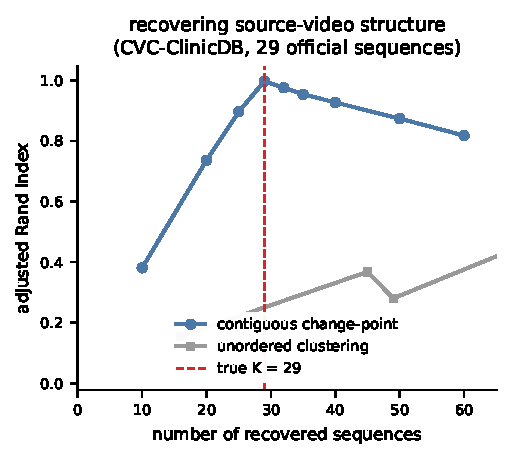
\includegraphics[width=0.52\textwidth]{fig5_sequence_recovery.pdf}
\caption{\textbf{Recovering source video structure.}
Agreement with CVC-ClinicDB's 29 official sequences for contiguous
change-point segmentation and for unordered clustering.}
\label{fig:recovery}
\end{figure}

\section*{Discussion}

% No subheadings, no Limitations section and no Conclusions section are
% permitted here. Limitations must be carried in the prose.
These findings concern the validity of a measurement instrument, not the
competence of the groups who built the datasets or the correctness of any
particular published number. The distinction is worth stating precisely,
because the two kinds of claim carry very different evidential burdens.

That CVC-300 is contained in CVC-ColonDB is not a statistical inference. The
images are identical under MD5 of their decoded pixel arrays and under a
256-bit perceptual hash at zero Hamming distance, and the two sets produce
mean Dice agreeing to within \IdentityMaxDiff{} when scored by five
independently trained architectures. Anyone can reproduce the check in
minutes. From that identity, one consequence follows deductively and requires
no experiment at all: a mean taken over CVC-300 and CVC-ColonDB as though they
were separate datasets counts \CVCThreeMatched{} images twice, and because
that block is \BlockGap{} Dice easier than the remainder of its parent, the
double counting is also biased upward rather than neutral. The same holds for
the \NDupesColon{} exact duplicates. These are properties of the artifacts,
and they hold for every study that has used them.

The magnitude of the leakage effect is a weaker claim and we state it as one.
It was measured for five architectures spanning four backbone families under a
single training recipe, and we did not retrain any published model. We
therefore cannot say what any specific reported score would become under a
leakage-free protocol. What makes extrapolation reasonable is that the
mechanism resides in the data and the partition rather than in the
architecture: a test frame whose sequence-mates appear in training is easier
for any model. That the effect appeared in all five architectures, and that
its size tracked dataset redundancy rather than the partitioning procedure,
supports that reading, but it remains an inference. The decomposition is
likewise approximate; using external performance to estimate the
training-diversity contribution assumes that contribution transfers
equally in and out of domain, which we cannot verify directly.

Our own prior work is subject to the same audit and we report its exposure
rather than exempting it. That study used the distributed CVC-ColonDB as an
external test set and cross-validated Kvasir-SEG at the image level, listing
the absence of patient identifiers as a limitation. The present measurement
puts that exposure at \InflationKvasir{} Dice, or
\InflationKvasirSigma$\sigma_{\mathrm{run}}$, which leaves its conclusions
intact but converts an acknowledged caveat into a quantity.

Two of our own methods failed and the failures are informative. Thresholding
a similarity graph and taking connected components, the obvious way to group
near-duplicates, percolates: by a correlation of 0.77 all 612 CVC-ClinicDB
frames collapse into one component, at which point the grouping is trivially
leak-safe and useless. Selecting the number of source sequences without
ground truth was also unstable, with a slope heuristic recovering 32 against a
true 29 on the full dataset but 27 and 25 against a true 15 on its halves. We
consequently certify leak-safety only for CVC-ClinicDB, where a published
table exists, and offer the recovered groupings for the remaining datasets as
a mitigation rather than a guarantee. A third limitation is that the
near-duplicate rates depend on a correlation threshold; the exact-duplicate
and containment results do not, which is why the argument rests on them.

The scope of the audit is also deliberately narrow. We examine the specific
bundle of artifacts that the prevailing protocol distributes, because that is
what published scores are computed on, and not the newer resources that have
since become available. Multi-centre collections such as
PolypGen~\citep{ali2023polypgen} and full-procedure video datasets such as
REAL-Colon~\citep{biffi2024realcolon} were assembled with provenance metadata
and centre or patient identifiers, which is precisely what the older datasets
lack, and they are better positioned to support the kind of partitioning we
recommend. Whether they contain comparable defects is an open question that
the released toolkit is intended to make cheap to answer; nothing in our
results speaks to it either way.

What follows for practice is modest and cheap. CVC-300 should not be reported
as a dataset independent of CVC-ColonDB, and an average over the suite should
not include both. Exact duplicates should be collapsed before scoring. Splits
should respect source sequences wherever a mapping exists or can be recovered,
and where it cannot, the resulting uncertainty should be stated rather than
assumed away. Effects smaller than a measured run-to-run noise floor should
not be interpreted, a point established previously~\citep{puri2026what} and
reinforced here, since the corrections we describe are several times that
floor while many published differences are not. To make this inexpensive we
release leakage-free splits, the recovered sequence labels, the contamination
matrix, per-image metrics for all \NRuns{} runs, and the audit code, so that
the checks reported here can be rerun on any new dataset before it enters
general use.

\section*{Methods}

\subsection*{Datasets and the distributed evaluation suite}
The audit covers the \NimagesTotal{} images of the five datasets that
constitute the standard suite: Kvasir-SEG~\citep{jha2020kvasirseg}
(\NKvasir{}), CVC-ClinicDB~\citep{bernal2015clinicdb} (\NClinic{}),
CVC-ColonDB~\citep{bernal2012colondb} (\NColon{}),
ETIS-LaribPolypDB~\citep{silva2014etis} (\NEtis{}) and CVC-300, the test
portion of EndoScene~\citep{vazquez2017endoscene} (\NCVCThree{}). We
additionally audit Kvasir-Sessile (\SessileN{}), which is distributed
separately; it is excluded from the suite total because, as reported in the
Results, its images are drawn from Kvasir-SEG and counting them there would
double-count them. The last
three were taken from the test bundle distributed with
PraNet~\citep{fan2020pranet}, which is the artifact the literature actually
evaluates on; we record its SHA-256 in the deposit so that the specific copy
audited here is identifiable. CVC-ClinicDB was obtained in its full 612-image
form rather than the 62-image subset in that bundle, which preserves the
original frame numbering and hence the official sequence table. Image data
are not redistributable and are not included in our release; Kvasir-SEG in
particular is licensed for research and educational use only.

\subsection*{Image-level duplicate detection}
Two deliberately dissimilar signals were computed per image so that neither
alone drives a conclusion, a precaution that proved necessary: one of the two
containments we report is invisible to exact hashing. Exact identity used the
MD5 digest of the decoded RGB pixel array, which is invariant to container
format and file metadata but not to any change in pixel values, including
lossy re-encoding between dataset releases. Near-duplicate similarity used
$64 \times 64$ mean-subtracted, L2-normalised greyscale thumbnails compared by
Pearson correlation, which is invariant to resolution, together with a
256-bit perceptual hash compared by Hamming distance, which tolerates mild
cropping and recompression. A pair was treated as the same frame only when
both criteria agreed, and all candidate matches above the reporting threshold
were written out with both file paths for inspection. Near-duplicate rates are
reported at $r > 0.90$, $0.95$ and $0.98$ because the rate is
threshold-dependent; the exact-duplicate and containment results involve no
threshold.

\subsection*{Recovering source video structure}
Frames belonging to one source sequence occupy a contiguous range of the
distributed numbering, so recovery was posed as segmentation of an ordered
stream. Each frame was represented by its normalised greyscale thumbnail
concatenated with per-channel colour histograms, each block L2-normalised so
that neither dominates. The frame order was partitioned into exactly $K$
contiguous segments minimising the total within-segment sum of squared
deviations, solved exactly by dynamic programming with prefix sums rather
than greedily. CVC-ClinicDB provides ground truth through its official
frame-range table of 29 sequences, against which recovery was scored by
adjusted Rand index, homogeneity, completeness and boundary F1 at tolerances
of zero, one and two frames. Unordered agglomerative clustering on the same
features, and connected components of a thresholded similarity graph, were
evaluated as alternatives; the latter percolates and was discarded.
Leak-safety was defined as completeness equal to one, that is no true
sequence split across groups, which an intentionally coarse segmentation
attains without requiring $K$ to be known.

\subsection*{Training protocol}
Five architectures spanning four backbone families were trained under one
recipe identical to that of ref.~\citep{puri2026what}: U-Net and U-Net++ with
ResNet-34 encoders, SegFormer-B0 and SegFormer-B2, and U-Net with a PVTv2-B2
encoder. Inputs were resized to $352 \times 352$ and optimised with AdamW
(learning rate $10^{-4}$, weight decay $10^{-4}$) under a cosine schedule,
batch size 16, at most 60 epochs with early stopping on validation Dice at a
patience of 15, minimising the sum of Dice and binary cross-entropy losses
under bfloat16 autocast. Predictions were resized to native resolution before
scoring. The released code of ref.~\citep{puri2026what} resolves image and
mask paths under the Kvasir-SEG naming convention only; rather than modify it,
which would weaken the claim that both studies share one recipe, we widened
the record builder through an adapter that honours explicit filenames when a
split file supplies them and otherwise delegates to the original function.
All \NRuns{} runs were executed on a single RTX 4090.

\subsection*{Paired comparison of split protocols}
Comparing the two protocols by their reported means would be confounded,
since the protocols necessarily induce different test folds and a difference
would mix leakage with the test sets containing different images. Both arms
were therefore constructed as five-fold partitions of the complete dataset, so
that every frame is held out exactly once under each protocol and the arms can
be compared image by image. Validation data were carved from whole groups
within the training portion so that the sequence-disjoint property holds for
validation as well. Inflation was summarised by the mean per-image difference
with percentile bootstrap intervals over $10^4$ resamples, and tested by
paired Wilcoxon signed-rank. Training-set sizes were matched as closely as
whole-sequence assignment permits (416--430 against 428--429 frames) so that
data volume is not a confound. All effects are reported both in Dice and in
units of $\sigma_{\mathrm{run}} = \SigmaRun{}$.

\subsection*{Content-free position prior}
For each fold, the training-fold masks were averaged on a $352 \times 352$
grid into a single probability map and binarised at the threshold maximising
mean Dice on the training fold. That one fixed shape was then scored against
every held-out mask. The predictor receives no image as input, so any Dice it
attains is attributable to the dataset's position and size prior alone.
Folds were the leak-free ones where a defensible grouping exists, and a plain
partition otherwise, which is noted in the results.

\section*{Data availability}

All derived data generated by this study are deposited at
\url{https://doi.org/10.5281/zenodo.23879374}: the full image index with
per-image pixel digests and
perceptual hashes, the cross-dataset contamination matrix and the list of
matched pairs, the exact-duplicate groups, within-dataset near-duplicate
rates, leakage-free split and fold definitions, recovered sequence labels for
CVC-ClinicDB with the official labels alongside for verification,
deduplicated test-set keep-lists, and per-image segmentation metrics for all
\NRuns{} training runs. The archived specification of CVC-ColonDB referred to
in the Results is available through the Internet Archive capture of the
creators' project page.

The underlying colonoscopy images are not redistributable and are not
included. They must be obtained from their original providers: Kvasir-SEG and
Kvasir-Sessile from the Simula datasets portal, CVC-ClinicDB and
ETIS-LaribPolypDB through their respective challenge sites, and CVC-ColonDB
and CVC-300 as distributed with PraNet. Kvasir-SEG is licensed for research
and educational purposes only. Every row of the released metrics identifies
its source image by filename so that results can be joined back to the
original data.

\section*{Code availability}

The audit toolkit and all analysis code are available at
\url{https://github.com/rishitpuri/polyp-benchmark-audit} and archived at
\url{https://doi.org/10.5281/zenodo.23879374}, including the
duplicate-detection and
sequence-recovery implementations, the split generators, the analysis scripts
that produce every reported number, and the figure scripts. Every value quoted
in this manuscript is generated from the released result files rather than
transcribed, so the text cannot diverge from the experiments.

\section*{Acknowledgements}
The author thanks the groups who created and released the datasets examined
here. This study was only possible because those resources were made public,
and the findings reported should be read as a consequence of the difficulty
of maintaining shared benchmark artifacts over more than a decade rather than
as a criticism of the considerable effort involved in producing them. No
funding was received for this work.

\section*{Author contributions}
R.P. is the sole author. R.P. conceived and designed the study, implemented
the audit and analysis software, performed all experiments, analysed and
interpreted the results, produced the figures and tables, prepared the data
and code release, and wrote the manuscript.

\section*{Competing interests}
The author is employed by Karl Storz Endoscopy-America, Inc. This study was
conceived and conducted independently of that employment. It uses only
publicly available datasets; no proprietary, employer-held or patient data
were used, and no employer resources, funding or personnel contributed to the
design, analysis, or reporting of the work. The employer had no role in the
decision to publish. The author declares no other competing interests.

\bibliographystyle{unsrtnat}
\bibliography{refs}

\end{document}
